%\documentclass[12pt]{article}
\documentclass[12pt,landscape]{article}


%packages
%\usepackage{latexsym}
\usepackage{graphicx}
\usepackage{wrapfig}
\usepackage{color}
\usepackage{amsmath}
\usepackage{dsfont}
\usepackage{placeins}
\usepackage{amssymb}
\usepackage{skull}
\usepackage{enumerate}
\usepackage{soul}
\usepackage{alphalph}
\usepackage{hyperref}
\usepackage{enumerate}
\usepackage{listings}
%\usepackage{fancyhdr}

%\fancyhf{} % clear all header and footers
%\renewcommand{\headrulewidth}{0pt} % remove the header rule
%\fancyfoot[LE, LO]{\thepage}


%\usepackage{pstricks,pst-node,pst-tree}

%\usepackage{algpseudocode}
%\usepackage{amsthm}
%\usepackage{hyperref}
%\usepackage{mathrsfs}
%\usepackage{amsfonts}
%\usepackage{bbding}
%\usepackage{listings}
%\usepackage{appendix}
\usepackage[margin=1in]{geometry}
%\geometry{papersize={8.5in,11in},total={6.5in,9in}}
%\usepackage{cancel}
%\usepackage{algorithmic, algorithm}

\definecolor{dkgreen}{rgb}{0,0.6,0}
\definecolor{gray}{rgb}{0.5,0.5,0.5}
\definecolor{mauve}{rgb}{0.58,0,0.82}
\lstset{ %
  language=R,                     % the language of the code
  basicstyle=\footnotesize,       % the size of the fonts that are used for the code
  numbers=left,                   % where to put the line-numbers
  numberstyle=\tiny\color{gray},  % the style that is used for the line-numbers
  stepnumber=1,                   % the step between two line-numbers. If it's 1, each line
                                  % will be numbered
  numbersep=5pt,                  % how far the line-numbers are from the code
  backgroundcolor=\color{white},  % choose the background color. You must add \usepackage{color}
  showspaces=false,               % show spaces adding particular underscores
  showstringspaces=false,         % underline spaces within strings
  showtabs=false,                 % show tabs within strings adding particular underscores
  frame=single,                   % adds a frame around the code
  rulecolor=\color{black},        % if not set, the frame-color may be changed on line-breaks within not-black text (e.g. commens (green here))
  tabsize=2,                      % sets default tabsize to 2 spaces
  captionpos=b,                   % sets the caption-position to bottom
  breaklines=true,                % sets automatic line breaking
  breakatwhitespace=false,        % sets if automatic breaks should only happen at whitespace
  title=\lstname,                 % show the filename of files included with \lstinputlisting;
                                  % also try caption instead of title
  keywordstyle=\color{black},      % keyword style
  commentstyle=\color{dkgreen},   % comment style
  stringstyle=\color{mauve},      % string literal style
  escapeinside={\%*}{*)},         % if you want to add a comment within your code
  morekeywords={*,...}            % if you want to add more keywords to the set
}

\newcommand{\qu}[1]{``#1''}
\newcommand{\spc}[1]{\\ \vspace{#1cm}}

\newcounter{probnum}
\setcounter{probnum}{1}

%create definition to allow local margin changes
\def\changemargin#1#2{\list{}{\rightmargin#2\leftmargin#1}\item[]}
\let\endchangemargin=\endlist 

%allow equations to span multiple pages
\allowdisplaybreaks

%define colors and color typesetting conveniences
\definecolor{gray}{rgb}{0.5,0.5,0.5}
\definecolor{black}{rgb}{0,0,0}
\definecolor{white}{rgb}{1,1,1}
\definecolor{blue}{rgb}{0.5,0.5,1}
\newcommand{\inblue}[1]{\color{blue}#1 \color{black}}
\definecolor{green}{rgb}{0.133,0.545,0.133}
\newcommand{\ingreen}[1]{\color{green}#1 \color{black}}
\definecolor{yellow}{rgb}{1,0.549,0}
\newcommand{\inyellow}[1]{\color{yellow}#1 \color{black}}
\definecolor{red}{rgb}{1,0.133,0.133}
\newcommand{\inred}[1]{\color{red}#1 \color{black}}
\definecolor{purple}{rgb}{0.58,0,0.827}
\newcommand{\inpurple}[1]{\color{purple}#1 \color{black}}
\definecolor{gray}{rgb}{0.5,0.5,0.5}
\newcommand{\ingray}[1]{\color{gray}#1 \color{black}}
\definecolor{backgcode}{rgb}{0.97,0.97,0.8}
\definecolor{Brown}{cmyk}{0,0.81,1,0.60}
\definecolor{OliveGreen}{cmyk}{0.64,0,0.95,0.40}
\definecolor{CadetBlue}{cmyk}{0.62,0.57,0.23,0}

%define new math operators
\DeclareMathOperator*{\argmax}{arg\,max~}
\DeclareMathOperator*{\argmin}{arg\,min~}
\DeclareMathOperator*{\argsup}{arg\,sup~}
\DeclareMathOperator*{\arginf}{arg\,inf~}
\DeclareMathOperator*{\convolution}{\text{\Huge{$\ast$}}}
\newcommand{\infconv}[2]{\convolution^\infty_{#1 = 1} #2}
%true functions

%%%% GENERAL SHORTCUTS

\makeatletter
\newalphalph{\alphmult}[mult]{\@alph}{26}
\renewcommand{\labelenumi}{(\alphmult{\value{enumi}})}
\renewcommand{\theenumi}{\AlphAlph{\value{enumi}}}
\makeatother
%shortcuts for pure typesetting conveniences
\newcommand{\bv}[1]{\boldsymbol{#1}}

%shortcuts for compound constants
\newcommand{\BetaDistrConst}{\dfrac{\Gamma(\alpha + \beta)}{\Gamma(\alpha)\Gamma(\beta)}}
\newcommand{\NormDistrConst}{\dfrac{1}{\sqrt{2\pi\sigma^2}}}

%shortcuts for conventional symbols
\newcommand{\tsq}{\tau^2}
\newcommand{\tsqh}{\hat{\tau}^2}
\newcommand{\sigsq}{\sigma^2}
\newcommand{\sigsqsq}{\parens{\sigma^2}^2}
\newcommand{\sigsqovern}{\dfrac{\sigsq}{n}}
\newcommand{\tausq}{\tau^2}
\newcommand{\tausqalpha}{\tau^2_\alpha}
\newcommand{\tausqbeta}{\tau^2_\beta}
\newcommand{\tausqsigma}{\tau^2_\sigma}
\newcommand{\betasq}{\beta^2}
\newcommand{\sigsqvec}{\bv{\sigma}^2}
\newcommand{\sigsqhat}{\hat{\sigma}^2}
\newcommand{\sigsqhatmlebayes}{\sigsqhat_{\text{Bayes, MLE}}}
\newcommand{\sigsqhatmle}{\sigsqhat_{\text{MLE}}}
\newcommand{\sigsqhatmap}{\sigsqhat_{\text{MAP}}}
\newcommand{\sigsqhatmmae}{\sigsqhat_{\text{MMAE}}}
\newcommand{\sigsqhatmmse}{\sigsqhat_{\text{MMSE}}}
\newcommand{\bSigma}{\bv{\Sigma}}
\newcommand{\bSigmainv}{\bSigma^{-1}}
\newcommand{\thetavec}{\bv{\theta}}
\newcommand{\thetahat}{\hat{\theta}}
\newcommand{\thetahatmm}{\hat{\theta}^{\mathrm{MM}}}
\newcommand{\thetahathatmm}{\thetahathat^{\mathrm{MM}}}
\newcommand{\thetahathatmle}{\thetahathat^{\mathrm{MLE}}}
\newcommand{\thetahatmle}{\hat{\theta}^{\mathrm{MLE}}}
\newcommand{\thetavechatmle}{\hat{\thetavec}^{\mathrm{MLE}}}
\newcommand{\muhat}{\hat{\mu}}
\newcommand{\musq}{\mu^2}
\newcommand{\muvec}{\bv{\mu}}
\newcommand{\muhatmle}{\muhat_{\text{MLE}}}
\newcommand{\lambdahat}{\hat{\lambda}}
\newcommand{\lambdahatmle}{\lambdahat_{\text{MLE}}}
\newcommand{\thetahatmap}{\hat{\theta}_{\mathrm{MAP}}}
\newcommand{\thetahatmmae}{\hat{\theta}_{\mathrm{MMAE}}}
\newcommand{\thetahatmmse}{\hat{\theta}_{\mathrm{MMSE}}}
\newcommand{\etavec}{\bv{\eta}}
\newcommand{\alphavec}{\bv{\alpha}}
\newcommand{\minimaxdec}{\delta^*_{\mathrm{mm}}}
\newcommand{\ybar}{\bar{y}}
\newcommand{\xbar}{\bar{x}}
\newcommand{\Xbar}{\bar{X}}
\newcommand{\iid}{~{\buildrel iid \over \sim}~}
\newcommand{\inddist}{~{\buildrel ind \over \sim}~}
\newcommand{\approxdist}{~{\buildrel \bv{\cdot} \over \sim}~}
\newcommand{\equalsindist}{~{\buildrel d \over =}~}
\newcommand{\loglik}[1]{\ell\parens{#1}}
\newcommand{\thetahatkminone}{\thetahat^{(k-1)}}
\newcommand{\thetahatkplusone}{\thetahat^{(k+1)}}
\newcommand{\thetahatk}{\thetahat^{(k)}}
\newcommand{\half}{\frac{1}{2}}
\newcommand{\third}{\frac{1}{3}}
\newcommand{\twothirds}{\frac{2}{3}}
\newcommand{\fourth}{\frac{1}{4}}
\newcommand{\fifth}{\frac{1}{5}}
\newcommand{\sixth}{\frac{1}{6}}

%shortcuts for vector and matrix notation
\newcommand{\A}{\bv{A}}
\newcommand{\At}{\A^T}
\newcommand{\Ainv}{\inverse{\A}}
\newcommand{\B}{\bv{B}}
\renewcommand{\b}{\bv{b}}
\renewcommand{\H}{\bv{H}}
\newcommand{\K}{\bv{K}}
\newcommand{\Kt}{\K^T}
\newcommand{\Kinv}{\inverse{K}}
\newcommand{\Kinvt}{(\Kinv)^T}
\newcommand{\M}{\bv{M}}
\newcommand{\Bt}{\B^T}
\newcommand{\Q}{\bv{Q}}
\newcommand{\Qt}{\Q^T}
\newcommand{\R}{\bv{R}}
\newcommand{\Rt}{\R^T}
\newcommand{\Z}{\bv{Z}}
\newcommand{\X}{\bv{X}}
\newcommand{\Xsub}{\X_{\text{(sub)}}}
\newcommand{\Xsubadj}{\X_{\text{(sub,adj)}}}
\newcommand{\I}{\bv{I}}
\newcommand{\Y}{\bv{Y}}
\newcommand{\sigsqI}{\sigsq\I}
\renewcommand{\P}{\bv{P}}
\newcommand{\Psub}{\P_{\text{(sub)}}}
\newcommand{\Pt}{\P^T}
\newcommand{\Pii}{P_{ii}}
\newcommand{\Pij}{P_{ij}}
\newcommand{\IminP}{(\I-\P)}
\newcommand{\Xt}{\bv{X}^T}
\newcommand{\XtX}{\Xt\X}
\newcommand{\XtXinv}{\parens{\Xt\X}^{-1}}
\newcommand{\XtXinvXt}{\XtXinv\Xt}
\newcommand{\XXtXinvXt}{\X\XtXinvXt}
\newcommand{\x}{\bv{x}}
\newcommand{\w}{\bv{w}}
\newcommand{\q}{\bv{q}}
\newcommand{\zerovec}{\bv{0}}
\newcommand{\onevec}{\bv{1}}
\newcommand{\oneton}{1, \ldots, n}
\newcommand{\yoneton}{y_1, \ldots, y_n}
\newcommand{\yonetonorder}{y_{(1)}, \ldots, y_{(n)}}
\newcommand{\Yoneton}{Y_1, \ldots, Y_n}
\newcommand{\iinoneton}{i \in \braces{\oneton}}
\newcommand{\onetom}{1, \ldots, m}
\newcommand{\jinonetom}{j \in \braces{\onetom}}
\newcommand{\xoneton}{x_1, \ldots, x_n}
\newcommand{\Xoneton}{X_1, \ldots, X_n}
\newcommand{\xt}{\x^T}
\newcommand{\y}{\bv{y}}
\newcommand{\yt}{\y^T}
\renewcommand{\c}{\bv{c}}
\newcommand{\ct}{\c^T}
\newcommand{\tstar}{\bv{t}^*}
\renewcommand{\u}{\bv{u}}
\renewcommand{\v}{\bv{v}}
\renewcommand{\a}{\bv{a}}
\newcommand{\s}{\bv{s}}
\newcommand{\yadj}{\y_{\text{(adj)}}}
\newcommand{\xjadj}{\x_{j\text{(adj)}}}
\newcommand{\xjadjM}{\x_{j \perp M}}
\newcommand{\yhat}{\hat{\y}}
\newcommand{\yhatsub}{\yhat_{\text{(sub)}}}
\newcommand{\yhatstar}{\yhat^*}
\newcommand{\yhatstarnew}{\yhatstar_{\text{new}}}
\newcommand{\z}{\bv{z}}
\newcommand{\zt}{\z^T}
\newcommand{\bb}{\bv{b}}
\newcommand{\bbt}{\bb^T}
\newcommand{\bbeta}{\bv{\beta}}
\newcommand{\beps}{\bv{\epsilon}}
\newcommand{\bepst}{\beps^T}
\newcommand{\e}{\bv{e}}
\newcommand{\Mofy}{\M(\y)}
\newcommand{\KofAlpha}{K(\alpha)}
\newcommand{\ellset}{\mathcal{L}}
\newcommand{\oneminalph}{1-\alpha}
\newcommand{\SSE}{\text{SSE}}
\newcommand{\SSEsub}{\text{SSE}_{\text{(sub)}}}
\newcommand{\MSE}{\text{MSE}}
\newcommand{\RMSE}{\text{RMSE}}
\newcommand{\SSR}{\text{SSR}}
\newcommand{\SST}{\text{SST}}
\newcommand{\JSest}{\delta_{\text{JS}}(\x)}
\newcommand{\Bayesest}{\delta_{\text{Bayes}}(\x)}
\newcommand{\EmpBayesest}{\delta_{\text{EmpBayes}}(\x)}
\newcommand{\BLUPest}{\delta_{\text{BLUP}}}
\newcommand{\MLEest}[1]{\hat{#1}_{\text{MLE}}}

%shortcuts for Linear Algebra stuff (i.e. vectors and matrices)
\newcommand{\twovec}[2]{\bracks{\begin{array}{c} #1 \\ #2 \end{array}}}
\newcommand{\threevec}[3]{\bracks{\begin{array}{c} #1 \\ #2 \\ #3 \end{array}}}
\newcommand{\fivevec}[5]{\bracks{\begin{array}{c} #1 \\ #2 \\ #3 \\ #4 \\ #5 \end{array}}}
\newcommand{\twobytwomat}[4]{\bracks{\begin{array}{cc} #1 & #2 \\ #3 & #4 \end{array}}}
\newcommand{\threebytwomat}[6]{\bracks{\begin{array}{cc} #1 & #2 \\ #3 & #4 \\ #5 & #6 \end{array}}}

%shortcuts for conventional compound symbols
\newcommand{\thetainthetas}{\theta \in \Theta}
\newcommand{\reals}{\mathbb{R}}
\newcommand{\complexes}{\mathbb{C}}
\newcommand{\rationals}{\mathbb{Q}}
\newcommand{\integers}{\mathbb{Z}}
\newcommand{\naturals}{\mathbb{N}}
\newcommand{\forallninN}{~~\forall n \in \naturals}
\newcommand{\forallxinN}[1]{~~\forall #1 \in \reals}
\newcommand{\matrixdims}[2]{\in \reals^{\,#1 \times #2}}
\newcommand{\inRn}[1]{\in \reals^{\,#1}}
\newcommand{\mathimplies}{\quad\Rightarrow\quad}
\newcommand{\mathlogicequiv}{\quad\Leftrightarrow\quad}
\newcommand{\eqncomment}[1]{\quad \text{(#1)}}
\newcommand{\limitn}{\lim_{n \rightarrow \infty}}
\newcommand{\limitN}{\lim_{N \rightarrow \infty}}
\newcommand{\limitd}{\lim_{d \rightarrow \infty}}
\newcommand{\limitt}{\lim_{t \rightarrow \infty}}
\newcommand{\limitsupn}{\limsup_{n \rightarrow \infty}~}
\newcommand{\limitinfn}{\liminf_{n \rightarrow \infty}~}
\newcommand{\limitk}{\lim_{k \rightarrow \infty}}
\newcommand{\limsupn}{\limsup_{n \rightarrow \infty}}
\newcommand{\limsupk}{\limsup_{k \rightarrow \infty}}
\newcommand{\floor}[1]{\left\lfloor #1 \right\rfloor}
\newcommand{\ceil}[1]{\left\lceil #1 \right\rceil}

%shortcuts for environments
\newcommand{\beqn}{\vspace{-0.25cm}\begin{eqnarray*}}
\newcommand{\eeqn}{\end{eqnarray*}}
\newcommand{\bneqn}{\vspace{-0.25cm}\begin{eqnarray}}
\newcommand{\eneqn}{\end{eqnarray}}
\newcommand{\benum}{\begin{itemize}}
\newcommand{\eenum}{\end{itemize}}

%shortcuts for mini environments
\newcommand{\parens}[1]{\left(#1\right)}
\newcommand{\squared}[1]{\parens{#1}^2}
\newcommand{\tothepow}[2]{\parens{#1}^{#2}}
\newcommand{\prob}[1]{\mathbb{P}\parens{#1}}
\newcommand{\probsub}[2]{\mathbb{P}_{#1}\parens{#2}}
\newcommand{\littleo}[1]{o\parens{#1}}
\newcommand{\bigo}[1]{O\parens{#1}}
\newcommand{\Lp}[1]{\mathbb{L}^{#1}}
\renewcommand{\arcsin}[1]{\text{arcsin}\parens{#1}}
\newcommand{\prodonen}[2]{\bracks{\prod_{#1=1}^n #2}}
\newcommand{\mysum}[4]{\sum_{#1=#2}^{#3} #4}
\newcommand{\sumonen}[2]{\sum_{#1=1}^n #2}
\newcommand{\infsum}[2]{\sum_{#1=1}^\infty #2}
\newcommand{\infprod}[2]{\prod_{#1=1}^\infty #2}
\newcommand{\infunion}[2]{\bigcup_{#1=1}^\infty #2}
\newcommand{\infinter}[2]{\bigcap_{#1=1}^\infty #2}
\newcommand{\infintegral}[2]{\int^\infty_{-\infty} #2 ~\text{d}#1}
\newcommand{\supthetas}[1]{\sup_{\thetainthetas}\braces{#1}}
\newcommand{\bracks}[1]{\left[#1\right]}
\newcommand{\braces}[1]{\left\{#1\right\}}
\newcommand{\angbraces}[1]{\left<#1\right>}
\newcommand{\set}[1]{\left\{#1\right\}}
\newcommand{\abss}[1]{\left|#1\right|}
\newcommand{\norm}[1]{\left|\left|#1\right|\right|}
\newcommand{\normsq}[1]{\norm{#1}^2}
\newcommand{\inverse}[1]{\parens{#1}^{-1}}
\newcommand{\rowof}[2]{\parens{#1}_{#2\cdot}}

%shortcuts for functionals
\newcommand{\realcomp}[1]{\text{Re}\bracks{#1}}
\newcommand{\imagcomp}[1]{\text{Im}\bracks{#1}}
\newcommand{\range}[1]{\text{range}\bracks{#1}}
\newcommand{\colsp}[1]{\text{colsp}\bracks{#1}}
\newcommand{\rowsp}[1]{\text{rowsp}\bracks{#1}}
\newcommand{\tr}[1]{\text{tr}\bracks{#1}}
\newcommand{\rank}[1]{\text{rank}\bracks{#1}}
\newcommand{\proj}[2]{\text{Proj}_{#1}\bracks{#2}}
\newcommand{\projcolspX}[1]{\text{Proj}_{\colsp{\X}}\bracks{#1}}
\newcommand{\median}[1]{\text{median}\bracks{#1}}
\newcommand{\mean}[1]{\text{mean}\bracks{#1}}
\newcommand{\dime}[1]{\text{dim}\bracks{#1}}
\renewcommand{\det}[1]{\text{det}\bracks{#1}}
\newcommand{\expe}[1]{\mathbb{E}\bracks{#1}}
\newcommand{\cexpe}[2]{\mathbb{E}\bracks{#1\,|\,#2}}
\newcommand{\expeabs}[1]{\expe{\abss{#1}}}
\newcommand{\expesub}[2]{\mathbb{E}_{#1}\bracks{#2}}
\newcommand{\cexpesub}[3]{\mathbb{E}_{#1}\bracks{#2~|~#3}}
\newcommand{\indic}[1]{\mathds{1}_{#1}}
\newcommand{\var}[1]{\mathbb{V}\text{ar}\bracks{#1}}
\newcommand{\cvar}[2]{\mathbb{V}\text{ar}\bracks{#1~|~#2}}
\newcommand{\mse}[1]{\mathbb{M}\text{SE}\bracks{#1}}
\newcommand{\sd}[1]{\mathbb{S}\text{D}\bracks{#1}}
\newcommand{\support}[1]{\mathbb{S}\text{upp}\bracks{#1}}
\newcommand{\cov}[2]{\mathbb{C}\text{ov}\bracks{#1, #2}}
\newcommand{\corr}[2]{\text{Corr}\bracks{#1, #2}}
\newcommand{\se}[1]{\text{SE}\bracks{#1}}
\newcommand{\seest}[1]{\hat{\text{SE}}\bracks{#1}}
\newcommand{\bias}[1]{\mathbb{B}\text{ias}\bracks{#1}}
\newcommand{\partialop}[2]{\dfrac{\partial}{\partial #1}\bracks{#2}}
\newcommand{\secpartialop}[2]{\dfrac{\partial^2}{\partial #1^2}\bracks{#2}}
\newcommand{\mixpartialop}[3]{\dfrac{\partial^2}{\partial #1 \partial #2}\bracks{#3}}

%shortcuts for functions
\renewcommand{\exp}[1]{\mathrm{exp}\parens{#1}}
\renewcommand{\cos}[1]{\text{cos}\parens{#1}}
\renewcommand{\sin}[1]{\text{sin}\parens{#1}}
\newcommand{\sign}[1]{\text{sign}\parens{#1}}
\newcommand{\are}[1]{\mathrm{ARE}\parens{#1}}
\newcommand{\natlog}[1]{\ln\parens{#1}}
\newcommand{\oneover}[1]{\frac{1}{#1}}
\newcommand{\overtwo}[1]{\frac{#1}{2}}
\newcommand{\overn}[1]{\frac{#1}{n}}
\newcommand{\oversqrtn}[1]{\frac{#1}{\sqrt{n}}}
\newcommand{\oneoversqrt}[1]{\oneover{\sqrt{#1}}}
\newcommand{\sqd}[1]{\parens{#1}^2}
\newcommand{\loss}[1]{\ell\parens{\theta, #1}}
\newcommand{\losstwo}[2]{\ell\parens{#1, #2}}
\newcommand{\cf}{\phi(t)}

%English language specific shortcuts
\newcommand{\ie}{\textit{i.e.} }
\newcommand{\AKA}{\textit{AKA} }
\renewcommand{\iff}{\textit{iff}}
\newcommand{\eg}{\textit{e.g.} }
\renewcommand{\st}{\textit{s.t.} }
\newcommand{\wrt}{\textit{w.r.t.} }
\newcommand{\mathst}{~~\text{\st}~~}
\newcommand{\mathand}{~~\text{and}~~}
\newcommand{\ala}{\textit{a la} }
\newcommand{\ppp}{posterior predictive p-value}
\newcommand{\dd}{dataset-to-dataset}

%shortcuts for distribution titles
\newcommand{\logistic}[2]{\mathrm{Logistic}\parens{#1,\,#2}}
\newcommand{\bernoulli}[1]{\mathrm{Bernoulli}\parens{#1}}
\newcommand{\betanot}[2]{\mathrm{Beta}\parens{#1,\,#2}}
\newcommand{\stdbetanot}{\betanot{\alpha}{\beta}}
\newcommand{\multnormnot}[3]{\mathcal{N}_{#1}\parens{#2,\,#3}}
\newcommand{\normnot}[2]{\mathcal{N}\parens{#1,\,#2}}
\newcommand{\classicnormnot}{\normnot{\mu}{\sigsq}}
\newcommand{\stdnormnot}{\normnot{0}{1}}
\newcommand{\uniform}[2]{\mathrm{U}\parens{#1,\,#2}}
\newcommand{\stduniform}{\uniform{0}{1}}
\newcommand{\exponential}[1]{\mathrm{Exp}\parens{#1}}
\newcommand{\geometric}[1]{\mathrm{Geometric}\parens{#1}}
\newcommand{\gammadist}[2]{\mathrm{Gamma}\parens{#1, #2}}
\newcommand{\negbin}[2]{\mathrm{NegBin}\parens{#1, #2}}
\newcommand{\poisson}[1]{\mathrm{Poisson}\parens{#1}}
\newcommand{\binomial}[2]{\mathrm{Binomial}\parens{#1,\,#2}}
\newcommand{\betabinomial}[3]{\mathrm{BetaBinomial}\parens{#1,\,#2,\,#3}}
\newcommand{\rayleigh}[1]{\mathrm{Rayleigh}\parens{#1}}
\newcommand{\multinomial}[3]{\mathrm{Multin}_{#1}\parens{#2,\,#3}}
\newcommand{\gammanot}[2]{\mathrm{Gamma}\parens{#1,\,#2}}
\newcommand{\cauchynot}[2]{\text{Cauchy}\parens{#1,\,#2}}
\newcommand{\invchisqnot}[1]{\text{Inv}\chisq{#1}}
\newcommand{\invscaledchisqnot}[2]{\text{ScaledInv}\ncchisq{#1}{#2}}
\newcommand{\invgammanot}[2]{\text{InvGamma}\parens{#1,\,#2}}
\newcommand{\chisq}[1]{\chi^2_{#1}}
\newcommand{\ncchisq}[2]{\chi^2_{#1}\parens{#2}}
\newcommand{\ncF}[3]{F_{#1,#2}\parens{#3}}

%shortcuts for PDF's of common distributions
\newcommand{\logisticpdf}[3]{\oneover{#3}\dfrac{\exp{-\dfrac{#1 - #2}{#3}}}{\parens{1+\exp{-\dfrac{#1 - #2}{#3}}}^2}}
\newcommand{\betapdf}[3]{\dfrac{\Gamma(#2 + #3)}{\Gamma(#2)\Gamma(#3)}#1^{#2-1} (1-#1)^{#3-1}}
\newcommand{\normpdf}[3]{\frac{1}{\sqrt{2\pi#3}}\exp{-\frac{1}{2#3}(#1 - #2)^2}}
\newcommand{\normpdfvarone}[2]{\dfrac{1}{\sqrt{2\pi}}e^{-\half(#1 - #2)^2}}
\newcommand{\chisqpdf}[2]{\dfrac{1}{2^{#2/2}\Gamma(#2/2)}\; {#1}^{#2/2-1} e^{-#1/2}}
\newcommand{\invchisqpdf}[2]{\dfrac{2^{-\overtwo{#1}}}{\Gamma(#2/2)}\,{#1}^{-\overtwo{#2}-1}  e^{-\oneover{2 #1}}}
\newcommand{\uniformdiscrete}[1]{\mathrm{Uniform}\parens{\braces{#1}}}
\newcommand{\exponentialpdf}[2]{#2\exp{-#2#1}}
\newcommand{\poissonpdf}[2]{\dfrac{e^{-#1} #1^{#2}}{#2!}}
\newcommand{\binomialpdf}[3]{\binom{#2}{#1}#3^{#1}(1-#3)^{#2-#1}}
\newcommand{\rayleighpdf}[2]{\dfrac{#1}{#2^2}\exp{-\dfrac{#1^2}{2 #2^2}}}
\newcommand{\gammapdf}[3]{\dfrac{#3^#2}{\Gamma\parens{#2}}#1^{#2-1}\exp{-#3 #1}}
\newcommand{\cauchypdf}[3]{\oneover{\pi} \dfrac{#3}{\parens{#1-#2}^2 + #3^2}}
\newcommand{\Gammaf}[1]{\Gamma\parens{#1}}

%shortcuts for miscellaneous typesetting conveniences
\newcommand{\notesref}[1]{\marginpar{\color{gray}\tt #1\color{black}}}

%%%% DOMAIN-SPECIFIC SHORTCUTS

%Real analysis related shortcuts
\newcommand{\zeroonecl}{\bracks{0,1}}
\newcommand{\forallepsgrzero}{\forall \epsilon > 0~~}
\newcommand{\lessthaneps}{< \epsilon}
\newcommand{\fraccomp}[1]{\text{frac}\bracks{#1}}

%Bayesian related shortcuts
\newcommand{\yrep}{y^{\text{rep}}}
\newcommand{\yrepisq}{(\yrep_i)^2}
\newcommand{\yrepvec}{\bv{y}^{\text{rep}}}


%Probability shortcuts
\newcommand{\SigField}{\mathcal{F}}
\newcommand{\ProbMap}{\mathcal{P}}
\newcommand{\probtrinity}{\parens{\Omega, \SigField, \ProbMap}}
\newcommand{\convp}{~{\buildrel p \over \rightarrow}~}
\newcommand{\convLp}[1]{~{\buildrel \Lp{#1} \over \rightarrow}~}
\newcommand{\nconvp}{~{\buildrel p \over \nrightarrow}~}
\newcommand{\convae}{~{\buildrel a.e. \over \longrightarrow}~}
\newcommand{\convau}{~{\buildrel a.u. \over \longrightarrow}~}
\newcommand{\nconvau}{~{\buildrel a.u. \over \nrightarrow}~}
\newcommand{\nconvae}{~{\buildrel a.e. \over \nrightarrow}~}
\newcommand{\convd}{~{\buildrel d \over \rightarrow}~}
\newcommand{\nconvd}{~{\buildrel d \over \nrightarrow}~}
\newcommand{\withprob}{~~\text{w.p.}~~}
\newcommand{\io}{~~\text{i.o.}}

\newcommand{\Acl}{\bar{A}}
\newcommand{\ENcl}{\bar{E}_N}
\newcommand{\diam}[1]{\text{diam}\parens{#1}}

\newcommand{\taua}{\tau_a}

\newcommand{\myint}[4]{\int_{#2}^{#3} #4 \,\text{d}#1}
\newcommand{\laplacet}[1]{\mathscr{L}\bracks{#1}}
\newcommand{\laplaceinvt}[1]{\mathscr{L}^{-1}\bracks{#1}}
\renewcommand{\max}[1]{\text{max}\braces{#1}}
\renewcommand{\min}[1]{\text{min}\braces{#1}}

\newcommand{\Vbar}[1]{\bar{V}\parens{#1}}
\newcommand{\expnegrtau}{\exp{-r\tau}}
\newcommand{\cprob}[2]{\prob{#1~|~#2}}
\newcommand{\cprobsub}[3]{\probsub{#1}{#2~|~#3}}
\newcommand{\ck}[2]{k\parens{#1~|~#2}}

%%% problem typesetting
\newcommand{\problem}{\vspace{0.2cm} \noindent {\large{\textsf{Problem \arabic{probnum}~}}} \addtocounter{probnum}{1}}
%\newcommand{\easyproblem}{\ingreen{\noindent \textsf{Problem \arabic{probnum}~}} \addtocounter{probnum}{1}}
%\newcommand{\intermediateproblem}{\noindent \inyellow{\textsf{Problem \arabic{probnum}~}} \addtocounter{probnum}{1}}
%\newcommand{\hardproblem}{\inred{\noindent \textsf{Problem \arabic{probnum}~}} \addtocounter{probnum}{1}}
%\newcommand{\extracreditproblem}{\noindent \inpurple{\textsf{Problem \arabic{probnum}~}} \addtocounter{probnum}{1}}

\newcommand{\easysubproblem}{\ingreen{\item}}
\newcommand{\intermediatesubproblem}{\inyellow{\item}}
\newcommand{\hardsubproblem}{\inred{\item}}
\newcommand{\extracreditsubproblem}{\inpurple{\item}}


\newcounter{numpts}
\setcounter{numpts}{0}


%\newcommand{\subquestionwithpoints}[1]{\addtocounter{numpts}{#1} \item \ingray{[#1 pt]}~~} %  / \arabic{numpts} pts
\newcommand{\subquestionwithpoints}[1]{\addtocounter{numpts}{#1} \item \ingray{[#1 pt / \arabic{numpts} pts]}~~}  
\newcommand{\truefalsesubquestionwithpoints}[1]{\subquestionwithpoints{#1} Record the letter(s) of all the following that are \textbf{true} in general. At least one will be true.}

\newcounter{nummin}
\setcounter{nummin}{0}

\usepackage{accents}
\newlength{\dhatheight}
\newcommand{\doublehat}[1]{%
    \settoheight{\dhatheight}{\ensuremath{\hat{#1}}}%
    \addtolength{\dhatheight}{-0.35ex}%
    \hat{\vphantom{\rule{1pt}{\dhatheight}}%
    \smash{\hat{#1}}}}
\newcommand{\thetahathat}{\doublehat{\theta}}

%\newcommand{\subquestionwithpoints}[1]{\addtocounter{numpts}{#1} \item \ingray{[#1 pt]}~~} %  / \arabic{numpts} pts
\newcommand{\timedsection}[1]{\addtocounter{nummin}{#1}{[#1min] \ingray{(and \arabic{nummin}min will have elapsed)}}}  
%\newcommand{\timedsection}[1]{\addtocounter{nummin}{#1}{[#1 min]}}

\usepackage{multicol}

\newcommand{\instr}{\small Your answer will consist of a lowercase string (e.g. \texttt{aebgd}) where the order of the letters does not matter. \normalsize}

\title{Math 341 / 650 Spring \the\year{} \\ Final Examination}
\author{Professor Adam Kapelner}

\date{Monday, May 24, \the\year{}}

\begin{document}
\maketitle

%\noindent Full Name \line(1,0){410}

\thispagestyle{empty}

\section*{Code of Academic Integrity}

\footnotesize
Since the college is an academic community, its fundamental purpose is the pursuit of knowledge. Essential to the success of this educational mission is a commitment to the principles of academic integrity. Every member of the college community is responsible for upholding the highest standards of honesty at all times. Students, as members of the community, are also responsible for adhering to the principles and spirit of the following Code of Academic Integrity.

Activities that have the effect or intention of interfering with education, pursuit of knowledge, or fair evaluation of a student's performance are prohibited. Examples of such activities include but are not limited to the following definitions:

\paragraph{Cheating} Using or attempting to use unauthorized assistance, material, or study aids in examinations or other academic work or preventing, or attempting to prevent, another from using authorized assistance, material, or study aids. Example: using an unauthorized cheat sheet in a quiz or exam, altering a graded exam and resubmitting it for a better grade, etc.
\\

\noindent By taking this exam, you acknowledge and agree to uphold this Code of Academic Integrity. \\

%\begin{center}
%\line(1,0){250} ~~~ \line(1,0){100}\\
%~~~~~~~~~~~~~~~~~~~~~signature~~~~~~~~~~~~~~~~~~~~~~~~~~~~~~~~~~~~~~~~~~~~~ date
%\end{center}

\normalsize

\section*{Instructions}
This exam is 110 minutes (variable time per question) and closed-book. You are allowed \textbf{three} pages (front and back) of a \qu{cheat sheet}, blank scrap paper and a graphing calculator. Please read the questions carefully. No food is allowed, only drinks. %If the question reads \qu{compute,} this means the solution will be a number otherwise you can leave the answer in \textit{any} widely accepted mathematical notation which could be resolved to an exact or approximate number with the use of a computer. I advise you to skip problems marked \qu{[Extra Credit]} until you have finished the other questions on the exam, then loop back and plug in all the holes. I also advise you to use pencil. The exam is 100 points total plus extra credit. Partial credit will be granted for incomplete answers on most of the questions. \fbox{Box} in your final answers. Good luck!

\pagebreak

%$\cprobsub{1}{X}{\theta} = \binomial{n}{\theta}$ with $n$ fixed, $\probsub{2}{\theta} = \betanot{\alpha}{\beta}$, $\cprobsub{3}{X}{\theta} = \poisson{\theta}$,  $\probsub{4}{\theta} = \gammanot{\alpha}{\beta}$, $\cprobsub{3}{X}{\theta} = \poisson{\theta}$


\problem\timedsection{17} Consider the case of the beta-binomial conjugate model with fixed $n$ under the prior of indifference. Let $X_*$ be the number of successes in $n_*$ future observations from the same process.

\vspace{-0.2cm}\benum\truefalsesubquestionwithpoints{26} 

\begin{multicols}{2}

\begin{enumerate}[(a)]
\item $\prob{\theta} \propto \betanot{0}{0}$
\item $\prob{\theta} = 1$
\item $\prob{\theta} \propto 1$
\item $\prob{\theta} \propto \binom{n}{x}\theta^x \tothepow{1-\theta}{n-x}$
\item $\prob{\theta} \propto \theta^x \tothepow{1-\theta}{n-x}$
\item $\prob{\theta} \propto \inverse{x! (n-x)!} \tothepow{\theta / (1-\theta)}{x}$
\item $\cprob{X}{\theta} = 1$
\item $\cprob{X}{\theta} \propto 1$
\item $\cprob{X}{\theta} \propto \binom{n}{x}\theta^x \tothepow{1-\theta}{n-x}$
\item $\cprob{X}{\theta} \propto \theta^x \tothepow{1-\theta}{n-x}$
\item $\cprob{X}{\theta} \propto \inverse{x! (n-x)!} \tothepow{\theta / (1-\theta)}{x}$
\item $\cprob{\theta}{X} = 1$
\item $\cprob{\theta}{X} \propto 1$
\item $\cprob{\theta}{X} \propto \binom{n}{x}\theta^x \tothepow{1-\theta}{n-x}$
\item $\cprob{\theta}{X} \propto \theta^x \tothepow{1-\theta}{n-x}$
\item $\cprob{\theta}{X} \propto \inverse{x! (n-x)!} \tothepow{\theta / (1-\theta)}{x}$
\item $\prob{X} = 1$
\item $\prob{X} \propto 1$
\item $\prob{X} \propto \binom{n}{x}\theta^x \tothepow{1-\theta}{n-x}$\\
%\item $\prob{X} \propto \theta^x \tothepow{1-\theta}{n-x}$
%\item $\prob{X} \propto \inverse{x! (n-x)!} \tothepow{\theta / (1-\theta)}{x}$

Be careful about $X$ and $X_*$ in the following problems:
\item $\cprob{X_*}{\theta} \propto \binom{n}{x_*}\theta^{x_*} \tothepow{1-\theta}{n-x_*}$
\item $\cprob{X_*}{\theta} \propto \theta^{x_*} \tothepow{1-\theta}{n-x_*}$
\item $\cprob{X_*}{\theta} \propto \inverse{x_*! (n-x_*)!} \tothepow{\theta / (1-\theta)}{x_*}$

\item $\cprob{X_*}{X} \propto \binom{n}{x_*}\theta^{x_*} \tothepow{1-\theta}{n-x_*}$
\item $\cprob{X_*}{X} \propto \theta^{x} \tothepow{1-\theta}{n-x}$
\item $\cprob{X_*}{X} \propto \theta^{x_*} \tothepow{1-\theta}{n-x_*}$
\item $\cprob{X_*}{X} \propto B(1 + x + x_*, 1 + n - x + n_* - x_*)$
\end{enumerate}

\end{multicols}
\eenum\instr\pagebreak

%%%%%%%%%%%%%%%%%%%%%%%%


\problem\timedsection{8} Recall the baseball batter example from class. Here, $\Xoneton \iid \bernoulli{\theta}$ where each $X_i$ is either a hit or not a hit. We are trying to infer $\theta$, his true probability of getting a hit (or his true \qu{batting average}). We employed the prior $\prob{\theta} = \betanot{\alpha = 78.7}{\beta = 224.8}$. Let $X = \sum_{i=1}^n X_i$. We collected the following data: $x = 11$ hits out of $n = 25$ at bats.

\vspace{-0.2cm}\benum\truefalsesubquestionwithpoints{10} 

\begin{enumerate}[(a)]
\item $\theta$ is considered fixed for every one of the $n$ at bats
\item $\prob{\theta}$ has the same support as the parameter space of $\cprob{X}{\theta}$
\item $\prob{\theta}$ has the same support as the support of $\cprob{\theta}{X}$
\item $\prob{\theta}$ is a principled uninformative prior even though it is not one of the three we explicitly studied in class
\item $\prob{\theta}$ has hyperparameters that were fit using the principle of indifference
\item With a different value of $n$, $\prob{\theta}$ could be considered uninformative
\item $\prob{\theta}$ can be sampled from using the function \texttt{pbeta}
\item $\prob{\theta}$ can be sampled from using the grid sampling algorithm
\item $\thetahatmmse$ is numerically closer to $\expe{\theta}$ than $\xbar = 11/25$ 
%$\thetahatmmAe$ is numerically closer to $\expe{\theta}$ than $\xbar = 11/25$
%$\thetahatmAP$ is numerically closer to $\expe{\theta}$ than $\xbar = 11/25$
\item A 95\% posterior predictive interval for the value of the next at bat could be computed by\\ ~[\texttt{qbeta}(2.5\%, $\alpha + x, \beta + n - x$), \texttt{qbeta}(97.5\%, $\alpha + x, \beta + n - x$)]
\end{enumerate}
\eenum\instr\pagebreak

%%%%%%%%%%%%%%%%%%%%%%%%


\problem\timedsection{10} We will continue with our discussion of the batter. But now we have a slightly different situation. There is reason to believe the player's $\theta$ changes during the course of his $n$ at bats (where $n$ is fixed). We denote this change point as $m$. Thus, for the first $m$ at bats, he bats with probability of getting a hit $\theta_0$ and for the remaining $n - m$ at bats, he bats with probability of getting a hit $\theta_1$ where $\theta_0 \neq \theta_1$. All at bats are considered independent. Since we are no longer interested in his lifetime career batting average, we have no need for the empirical Bayes prior of the previous problem. We now use Laplace's prior for $\theta_0$ and $\theta_1$. Since we have no strong feeling of where the change point is, we use Laplace's prior as well there. We are interested in inference for all unknown parameters using the data $x := \bracks{\xoneton}$ where each value is 1 if there is a hit at time $t$ or 0 if not.

\vspace{-0.2cm}\benum\truefalsesubquestionwithpoints{14} 

\begin{enumerate}[(a)]
\item $X_1, \ldots, X_m \iid \binomial{m}{\theta_0}$
\item The unknown parameters are $\theta_0, \theta_1, m, n, t$
\item The unknown parameters are $\theta_0, \theta_1, m, n$
\item The unknown parameters are $\theta_0, \theta_1, m$
\item $\theta_0 + \theta_1 = 1$
\item The shrinkage $\rho$ for posterior expectation of $\theta_0$ can be computed as $m\theta_0 + (n-m)\theta_1$
\item $\prob{\theta_0} = 1$
\item $\prob{\theta_1} = 1$
\item $\prob{m} = 1$
\item The likelihood of the data is the same if $m = 0$ as if $m = n$
\item The posterior is the same value if calculated at $m = 0$ and $m = n$
\item If $X_*$ denotes the random variable (rv) of only the next at bat, then $X_*$ is a bernoulli random variable
\item If $X_*$ denotes the rv of the next $n_* > 1$ at bats, then $X_*$ is a binomial random variable if the data and $\theta_1$ is known
\item If $X_*$ denotes the rv of the next $n_* > 1$ at bats, then $X_*$ is a betabinomial random variable if the data and $m$ is known
\end{enumerate}
\eenum\instr\pagebreak

%%%%%%%%%%%%%%%%%%%%%%%%


\problem\timedsection{11} \ingray{We will continue with our discussion of the batter. But now we have a slightly different situation. There is reason to believe the player's $\theta$ changes during the course of his $n$ at bats (where $n$ is fixed). We denote this change point as $m$. Thus, for the first $m$ at bats, he bats with probability of getting a hit $\theta_0$ and for the remaining $n - m$ at bats, he bats with probability of getting a hit $\theta_1$ where $\theta_0 \neq \theta_1$. All at bats are considered independent. Since we are no longer interested in his lifetime career batting average, we have no need for the empirical Bayes prior of the previous problem. We now use Laplace's prior for $\theta_0$ and $\theta_1$. Since we have no strong feeling of where the change point is, we use Laplace's prior as well there. We are interested in inference for all unknown parameters using the data $x := \bracks{\xoneton}$ where each value is 1 if there is a hit at time $t$ or 0 if not.} Letting $a := \sum_{i=1}^m x_i$ and $b = \sum_{i = m + 1}^n x_i$ (where $a$ is defined to be zero if $m=0$ and $b$ is defined to be zero if $m=n$), the likelihood of the data can be written as:

\beqn
\cprob{X}{\theta_0, \theta_1, m} = \binom{m}{a} \theta_0^a (1-\theta_0)^{m-a}  \binom{n-m}{b} \theta_1^b (1-\theta_1)^{n-m-b}.
\eeqn

\vspace{-0.2cm}\benum\truefalsesubquestionwithpoints{8} 

\begin{enumerate}[(a)]
\item The likelihood of the data can be decomposed as $\cprob{X}{\theta_0, \theta_1, m} = \cprob{X_1, \ldots, X_m}{\theta_0, m} \cprob{X_{m+1}, \ldots, X_n}{\theta_1, m}$
\item The likelihood of the data can be decomposed as $\cprob{X}{\theta_0, \theta_1, m} = \cprob{X_1, \ldots, X_m}{\theta_0} \cprob{X_{m+1}, \ldots, X_n}{\theta_1} \cprob{X}{m}$
\item $\cprob{\theta_0, \theta_1, m}{X} \propto \cprob{X}{\theta_0, \theta_1, m}$
\item $k(\theta_0, \theta_1, m~|~X) = \cprob{X}{\theta_0, \theta_1, m}$ where $k$ denotes the irreducible kernel of the distribution
\item $\cprob{\theta_0}{X, \theta_1, m} = \betanot{a + 1}{m - a + 1}$
\item $\cprob{\theta_1}{X, \theta_0, m} = \betanot{b + 1}{m - b + 1}$
\item $\cprob{m}{X, \theta_0, \theta_1} = \betabinomial{n}{\theta_0}{\theta_1}$
\item $k(m~|~X, \theta_0, \theta_1) = \cprob{m}{X, \theta_0, \theta_1}$ where $k$ denotes the irreducible kernel of the distribution
\end{enumerate}
\eenum\instr\pagebreak

%%%%%%%%%%%%%%%%%%%%%%%%


\problem\timedsection{6} \ingray{\small We will continue with our discussion of the batter. But now we have a slightly different situation. There is reason to believe the player's $\theta$ changes during the course of his $n$ at bats (where $n$ is fixed). We denote this change point as $m$. Thus, for the first $m$ at bats, he bats with probability of getting a hit $\theta_0$ and for the remaining $n - m$ at bats, he bats with probability of getting a hit $\theta_1$ where $\theta_0 \neq \theta_1$. All at bats are considered independent. Since we are no longer interested in his lifetime career batting average, we have no need for the empirical Bayes prior of the previous problem. We now use Laplace's prior for $\theta_0$ and $\theta_1$. Since we have no strong feeling of where the change point is, we use Laplace's prior as well there. We are interested in inference for all unknown parameters using the data $x := \bracks{\xoneton}$ where each value is 1 if there is a hit at time $t$ or 0 if not.Letting $a := \sum_{i=1}^m x_i$ and $b = \sum_{i = m + 1}^n x_i$ (where $a$ is defined to be zero if $m=0$ and $b$ is defined to be zero if $m=n$),} \normalsize  we can show that:

\beqn
\cprob{\theta_0}{X, \theta_1, m} &=& \betanot{a + 1}{m - a + 1}, \\
\cprob{\theta_1}{X, \theta_0, m} &=& \betanot{b + 1}{n - m - b + 1},\\
k(m~|~X, \theta_0, \theta_1) &\propto& \binom{m}{a} \theta_0^a (1-\theta_0)^{m-a}  \binom{n-m}{b} \theta_1^b (1-\theta_1)^{-m-b}.
\eeqn

\vspace{-0.2cm}\benum\truefalsesubquestionwithpoints{13} 

\begin{enumerate}[(a)]
\item $\cprob{m}{X, \theta_0, \theta_1}$ can be solved for in closed form and thus can be computed exactly
\item Regardless of whether (a) is true, $\cprob{m}{X, \theta_0, \theta_1}$ can be sampled from using a grid sampler
\item Regardless of whether (b) is true, a grid sampler for $\cprob{m}{X, \theta_0, \theta_1}$ will suffer since we do not know how to set the minimum and maximum sizes of $m$ nor the grid resolution $\Delta$
\item Using the information above, you can sample from $\cprob{\theta_0, \theta_1, m}{X}$ using a systematic sweep Gibbs sampler which will eventually converge
\item Assume the Gibbs sampler will converge, starting at $\theta_0 = 0$, $\theta_1 = 0$ and $m = 0$ will allow for convergence
\end{enumerate}
\eenum\instr\pagebreak

%%%%%%%%%%%%%%%%%%%%%%%%


\problem\timedsection{4} In our dataset, $n = 30$. Using the three conditional distributions from the previous problem within a systematic sweep Gibbs sampler running for $S=100,000$ iterations, we find that the Gibbs sampler burns in almost immediately, so we set $B=10$. We now wish to assess sample dependence. Here are the autocorrelation plots for $\theta_0$ (top), $\theta_1$ (middle) and $m$ (bottom):

\vspace{-0.3cm}
\begin{figure}[h]
\centering
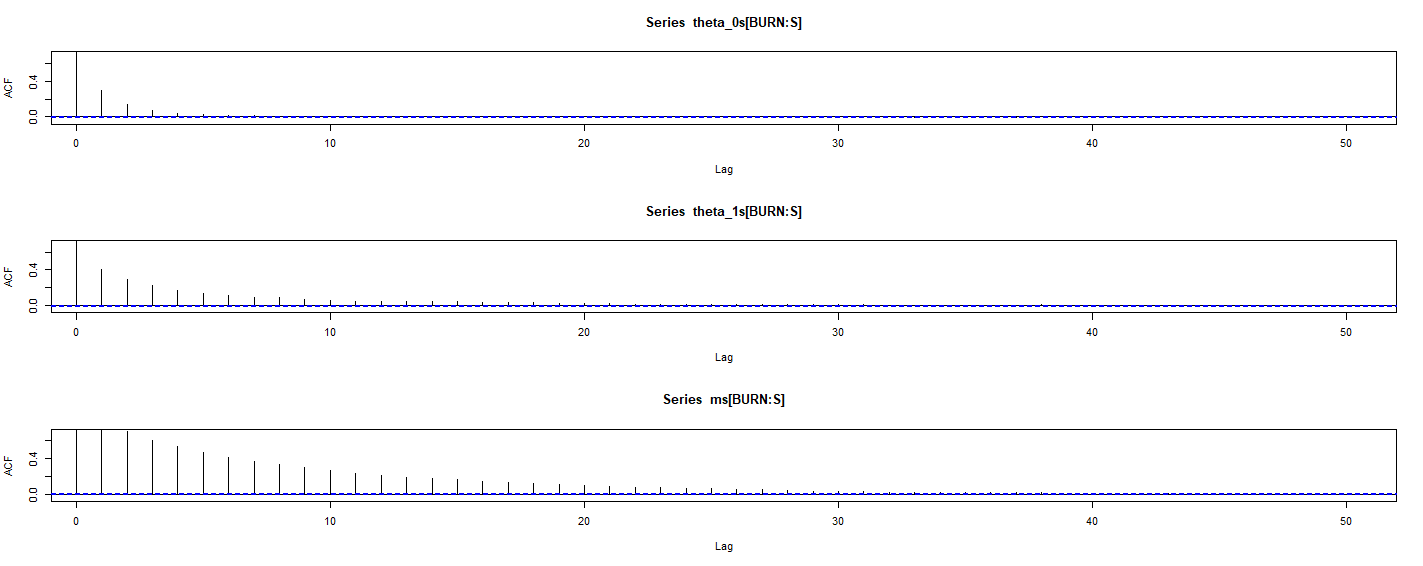
\includegraphics[width=9in]{acfs.png}
\end{figure}

\vspace{-0.2cm}\benum\truefalsesubquestionwithpoints{4} 

\begin{enumerate}[(a)]
%\item The samples never become independent enough to be used for inference
\item The samples of $\theta_0$ become independent of each other more quickly than the samples of $\theta_1$ which become more quickly independent than the samples of $m$
\item We can thin the Gibbs chain every 10 iterations to arrive at iid samples from the burned and thinned chain
\item We can thin the Gibbs chain every 40 iterations to arrive at iid samples from the burned and thinned chain
\item We cannot tell when to thin the Gibbs chain from these plots
\end{enumerate}
\eenum\instr\pagebreak

%%%%%%%%%%%%%%%%%%%%%%%%


\problem\timedsection{6} \ingray{In our dataset, $n = 30$. Using the three conditional distributions from the previous problem within a systematic sweep Gibbs sampler running for $S=100,000$ iterations, we find that the Gibbs sampler burns in almost immediately, so we set $B=10$.} We thinned every 40 iterations. Below is a histogram of the burned and thinned samples of $\theta_0$ (top) and $\theta_1$ (bottom):

\vspace{-0.3cm}
\begin{figure}[h]
\centering
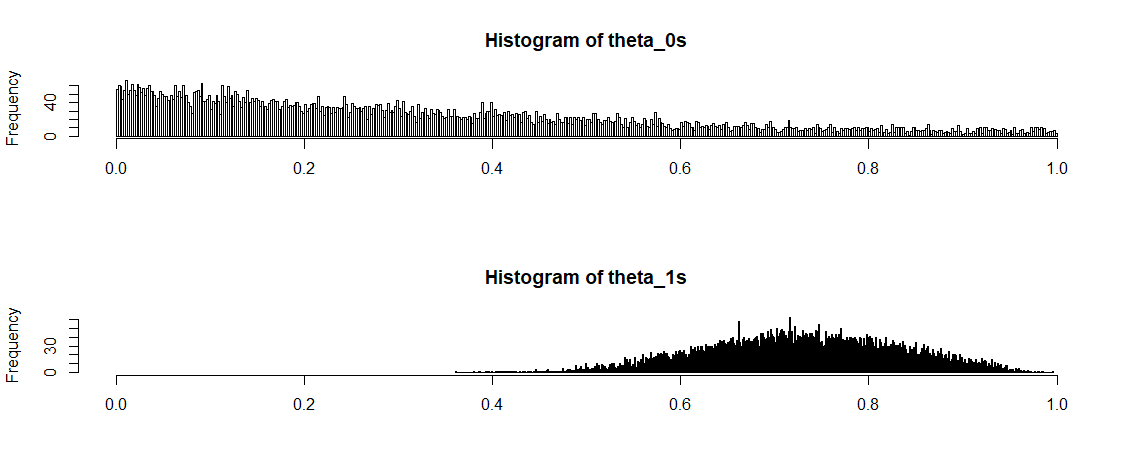
\includegraphics[width=8in]{thetas.png}
\end{figure}

\vspace{-1.2cm}\benum\truefalsesubquestionwithpoints{6} 

\begin{enumerate}[(a)]
%\item The samples never become independent enough to be used for inference
\item There are 11,110 samples for $\theta_0$
\item There are a different number of samples for $\theta_0$ and $\theta_1$
\item It is likely that $\cvar{\theta_0}{X} > \cvar{\theta_1}{X}$
\item It is likely that $m$ is small relative to $n-m$
\item It is not possible to approiximate a point estimate for $\theta_0$ given this illustration
\item It is likely that $\theta_1 > \theta_0$
%\item A 95\% CR for $\theta_1$ is approximately [0.025,~0.975]
\end{enumerate}
\eenum\instr\pagebreak

%%%%%%%%%%%%%%%%%%%%%%%%


\problem\timedsection{6} \ingray{In our dataset, $n = 30$. Using the three conditional distributions from the previous problem within a systematic sweep Gibbs sampler running for $S=100,000$ iterations, we find that the Gibbs sampler burns in almost immediately, so we set $B=10$. We thinned every 40 iterations. Below is a histogram of the burned and thinned samples of $\theta_0$ (top) and $\theta_1$ (bottom):}

\vspace{-0.3cm}
\begin{figure}[h]
\centering
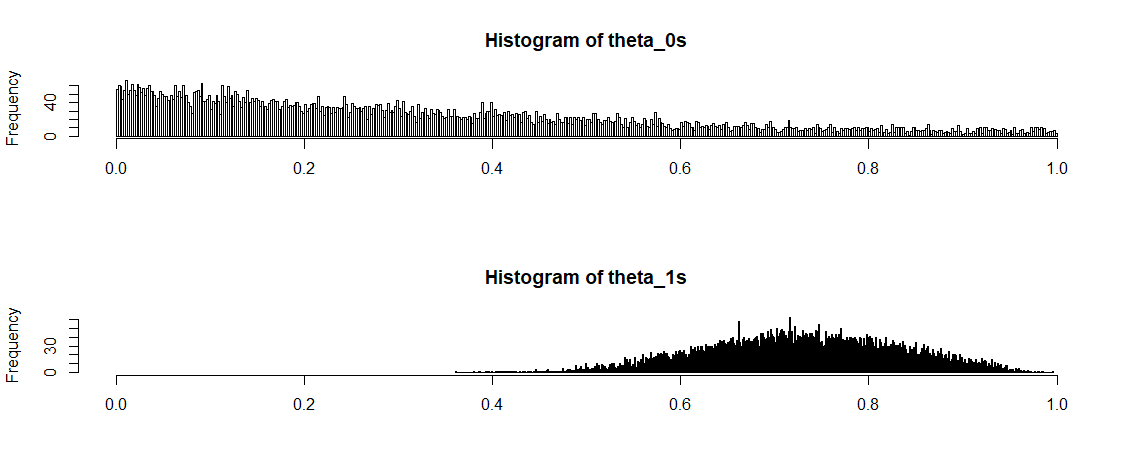
\includegraphics[width=8in]{thetas.png}
\end{figure}

\vspace{-1.2cm}\benum\truefalsesubquestionwithpoints{5} 

\begin{enumerate}[(a)]
\item The MMSE estimate for $\theta_0$ is near 0.3
\item The MAP estimate for $\theta_0$ is definitely zero
\item The MMSE estimate for $\theta_1$ is slightly higher than 0.7
\item The MMAE estimate for $\theta_1$ is slightly higher than 0.7
\item The MAP estimate for $\theta_1$ is likely near the MMSE estimate for $\theta_1$
\end{enumerate}
\eenum\instr\pagebreak

%%%%%%%%%%%%%%%%%%%%%%%%

\problem\timedsection{6} \ingray{In our dataset, $n = 30$. Using the three conditional distributions from the previous problem within a systematic sweep Gibbs sampler running for $S=100,000$ iterations, we find that the Gibbs sampler burns in almost immediately, so we set $B=10$. We thinned every 40 iterations.} Below is a histogram of the burned and thinned samples of $m$:

\vspace{-0.3cm}
\begin{figure}[h]
\centering
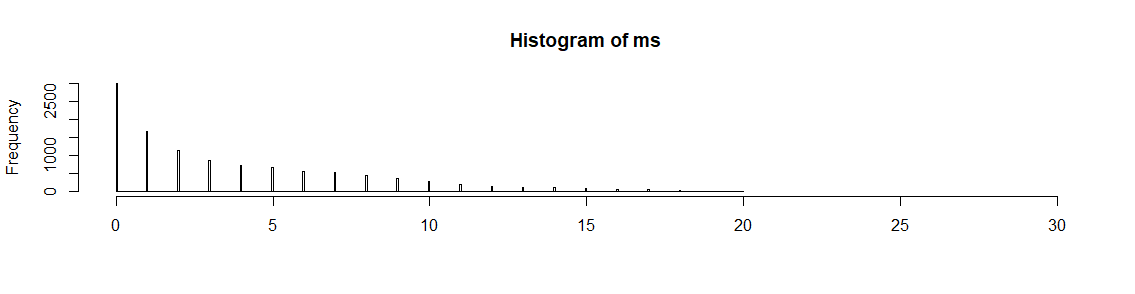
\includegraphics[width=8in]{ms.png}
\end{figure}

\vspace{-1.2cm}\benum\truefalsesubquestionwithpoints{7} 

\begin{enumerate}[(a)]
\item The MMSE estimate for $m$ must be a value in the set $\braces{0, 1, \ldots, n}$
\item The MMSE estimate for $m$ is near 4
\item The MAP estimate for $m$ is definitely zero
\item If we were to test that $m > 15$, the null hypothesis would likely be rejected
\item The 95\% credible region for $m$ is $\braces{0, 1, \ldots, 14}$ and this means the true value of $m$ is one of the values in the set $\braces{0, 1, \ldots, 14}$
\item Since there is no mass in $\cprob{m}{X}$ above $m=20$, this means it is likely we burned too soon in our Gibbs chain
\item Since there is no mass in $\cprob{m}{X}$ above $m=20$, this means it is likely we did not thin the Gibbs chain appropriately
\end{enumerate}
\eenum\instr\pagebreak

%%%%%%%%%%%%%%%%%%%%%%%%

\problem\timedsection{5} \ingray{In our dataset, $n = 30$. Using the three conditional distributions from the previous problem within a systematic sweep Gibbs sampler running for $S=100,000$ iterations, we find that the Gibbs sampler burns in almost immediately, so we set $B=10$. We thinned every 40 iterations.} We are interested in the difference in probability of getting a hit in the assumed two periods of the players batting. Below is a histogram of the samples of the ratio of $\theta_0 / \theta_1$

\vspace{-0.3cm}
\begin{figure}[h]
\centering
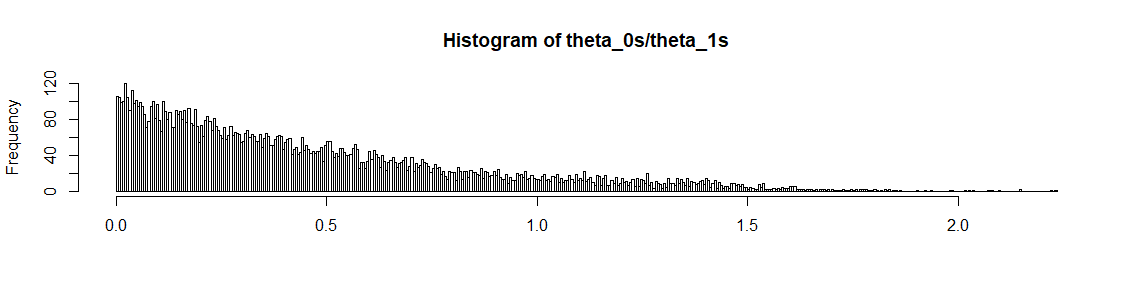
\includegraphics[width=8in]{ratio.png}
\end{figure}

\vspace{-1.2cm}\benum\truefalsesubquestionwithpoints{3} 

\begin{enumerate}[(a)]
\item If we were to test $H_a: \theta_0 \neq \theta_1$, the null hypothesis would be rejected since there is little mass in vicinity of 1.0 in the plot above
\item If we were to test $H_a: \theta_0 \neq \theta_1$, the null hypothesis would be rejected since there is little mass in vicinity of 0.0 in the plot above
\item If we were to test $H_a: \theta_0 \neq \theta_1$, the null hypothesis would be rejected since there is little mass in the right tail
\end{enumerate}
\eenum\instr\pagebreak

%%%%%%%%%%%%%%%%%%%%%%%%


\problem\timedsection{17} Consider the iid normal model where both the mean and variance are unknown. After a long derivation we find that $\cprob{\theta, \sigsq}{X} = \text{NormInvGamma}(\mu = \xbar, \lambda = n, \alpha = n/2, \beta = (n-1)s^2 / 2)$.

\vspace{-0.2cm}\benum\truefalsesubquestionwithpoints{17} 

\begin{enumerate}[(a)]
\item We used Jeffrey's priors for both the prior on $\theta$ and the prior on $\sigsq$
\item The prior on $\theta$ and the prior on $\sigsq$ are the same distribution
\item The prior we used is an informative prior
\item It is possible to arrive at this posterior if $\prob{\theta} = \normnot{\mu_0}{\tausq}$ for specific values of the constants $\mu_0$ and $\tausq$
\item $\cprob{\theta, \sigsq}{X} = \cprob{\theta}{X,\sigsq}\cprob{\sigsq}{X}$ where $\cprob{\sigsq}{X} = \invgammanot{\alpha}{\beta}$
\item $\cprob{\theta, \sigsq}{X} = \cprob{\theta}{X,\sigsq}\cprob{\sigsq}{X}$ where $\cprob{\theta}{X,\sigsq}= \normnot{\mu}{\lambda}$
\item $\cprob{\theta, \sigsq}{X} = \cprob{\sigsq}{X, \theta}\cprob{\theta}{X}$ where $\cprob{\sigsq}{X, \theta}$ has an inverse gamma distribution
\item $\cprob{\theta, \sigsq}{X} = \cprob{\sigsq}{X, \theta}\cprob{\theta}{X}$ where $\cprob{\theta}{X}$ has a normal distribution

\item You can sample from $\cprob{\theta, \sigsq}{X}$ exactly by first sampling from $\cprob{\sigsq}{X}$ to obtain $\sigsq_{samp}$ and then sampling $\theta_{samp}$ from $\cprob{\theta}{X,\sigsq = \sigsq_{samp}}$ and returning the pair $\angbraces{\theta_{samp}, \sigsq_{samp}}$
\item You can sample from $\cprob{\theta, \sigsq}{X}$ exactly by first sampling from $\cprob{\sigsq}{X, \theta = \theta_0}$ to obtain $\sigsq_{samp}$ and then sampling $\theta_{samp}$ from $\cprob{\theta}{X,\sigsq = \sigsq_{samp}}$ and returning the pair $\angbraces{\theta_{samp}, \sigsq_{samp}}$ as long as $\theta_0$ is in the parameter space of the parametric model which in our case is any real number

\item You can sample from $\cprob{\theta, \sigsq}{X}$ exactly by first sampling from $\cprob{\theta}{X}$ to obtain $\theta_{samp}$ and then sampling $\sigsq_{samp}$ from $\cprob{\sigsq}{X,\theta = \theta_{samp}}$ and returning the pair $\angbraces{\theta_{samp}, \sigsq_{samp}}$
\item You can sample from $\cprob{\theta, \sigsq}{X}$ exactly by first sampling from $\cprob{\theta}{X, \theta = \sigsq_0}$ to obtain $\theta_{samp}$ and then sampling $\sigsq_{samp}$ from $\cprob{\sigsq}{X,\theta = \theta_{samp}}$ and returning the pair $\angbraces{\theta_{samp}, \sigsq_{samp}}$ as long as $\sigsq_0$ is in the parameter space of the parametric model which in our case is any positive real number

\item $\int_0^\infty \cprob{\theta, \sigsq}{X} d\sigsq$ is a known distribution
\item $\int_\reals \int_0^\infty \cprob{\theta, \sigsq}{X} d\sigsq d\theta$ is a known distribution
\item The estimate $\cexpe{\theta}{X}$ has no shrinkage to the prior expectation
\item $\cexpe{\theta}{X} = \cexpe{\theta}{X, \sigsq}$ for any value of $n$ and any value of $\sigsq$ in its parameter space
\item $\cexpe{\sigsq}{X} = \cexpe{\sigsq}{X, \theta}$ for any value of $n$ and any value of $\theta$ in its parameter space
\end{enumerate}
\eenum\instr\pagebreak

%%%%%%%%%%%%%%%%%%%%%%%%


\problem\timedsection{9} \ingray{Consider the iid normal model where both the mean and variance are unknown. After a long derivation we find that $\cprob{\theta, \sigsq}{X} = \text{NormInvGamma}(\mu = \xbar, \lambda = n, \alpha = n/2, \beta = (n-1)s^2 / 2)$.} We sample $S = 10,000$ realizations from this posterior $\mathcal{S} := \braces{\angbraces{\theta_1, \sigsq_1}, \angbraces{\theta_2, \sigsq_2}, \ldots, \angbraces{\theta_S, \sigsq_S}}$. A sample of 1,000 points $\in \mathcal{S}$ is displayed below where $\theta$ is on the x-axis and $\sigsq$ is on the y-axis.



\vspace{-0.3cm}
\begin{figure}[h]
\centering
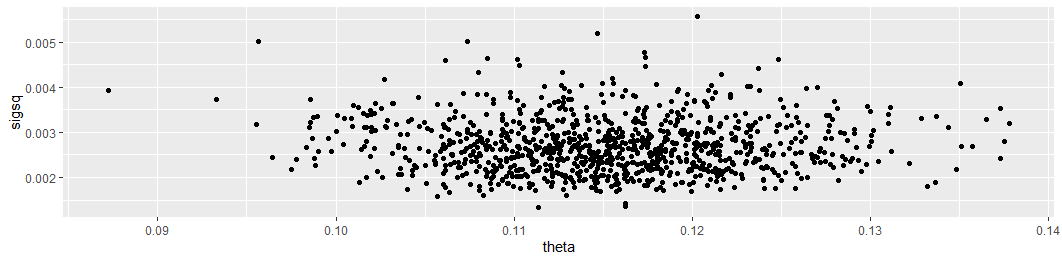
\includegraphics[width=8in]{theta_sigsqs.png}
\end{figure}

\vspace{-0.2cm}\benum\truefalsesubquestionwithpoints{9} 

\begin{enumerate}[(a)]
\item A 95\% HDR region would be rectangular in shape
\item $\sigsqhatmmse$ can be approximated from this plot
\item $\sigsqhatmmse$ can be approximated with $\oneover{S} \sum_{t=1}^S \sigsq_t$
\item A 95\% CR for $\cprob{\sigsq}{X}$ can be approximated from this plot
\item A 95\% CR for $\cprob{\sigsq}{X, \theta}$ can be approximated from this plot for every value of $\theta$ in the parameter space of $\theta$
\item During a test of $\theta > 0.90$, the null hypothesis would likely be rejected
\item During a test of $\sigma > 0.045$, the null hypothesis would likely be rejected
\item Sampling a future observation $x_*$ given the data can be done as follows: first draw a random sample $\angbraces{\theta_s, \sigsq_s}$ from the set $\mathcal{S}$ and then draw $x_*$ via \texttt{rnorm}($\theta_s, \sqrt{\sigsq_s}$)
\item Sampling a future observation $x_*$ given the data can be done as follows: first draw a random sample $\angbraces{\theta_s, \sigsq_s}$ from the set $\mathcal{S}$ and then draw $x_*$ via \texttt{rt.scaled}($n-1,\theta_s, \sqrt{\sigsq_s}$)
\end{enumerate}
\eenum\instr\pagebreak

%%%%%%%%%%%%%%%%%%%%%%%%


\problem\timedsection{5} \ingray{Consider the iid normal model where both the mean and variance are unknown. After a long derivation we find that $\cprob{\theta, \sigsq}{X} = \text{NormInvGamma}(\mu = \xbar, \lambda = n, \alpha = n/2, \beta = (n-1)s^2 / 2)$. We sample $S = 10,000$ realizations from this posterior $\mathcal{S} := \braces{\angbraces{\theta_1, \sigsq_1}, \angbraces{\theta_2, \sigsq_2}, \ldots, \angbraces{\theta_S, \sigsq_S}}$.} We now also plot a best fit line in blue which tries to approximate $\cexpe{\sigsq}{X, \theta}$ over all values of $\theta$ on the plot. To see the line clearer, we zoom in to display $\sigsq$ values between 0.002 and 0.003 (which is different from the previous plot that showed $\sigsq$ values between 0.002 and 0.006):



\vspace{-0.3cm}
\begin{figure}[h]
\centering
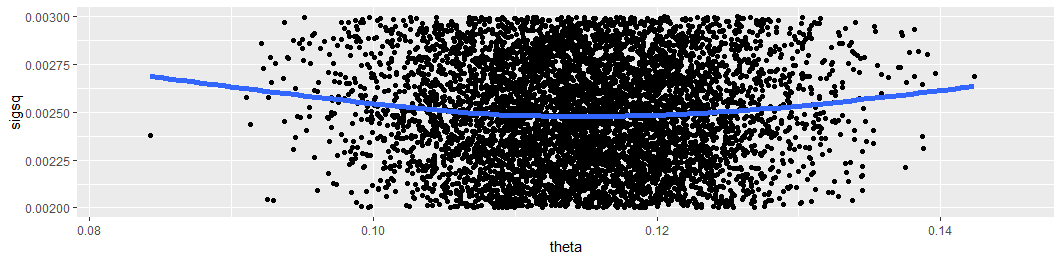
\includegraphics[width=8in]{best_fit_line.png}
\end{figure}

\vspace{-0.2cm}\benum\truefalsesubquestionwithpoints{3} 

\begin{enumerate}[(a)]
\item This line should be flat (i.e. slope zero) but it is curved only due to random variation (if we had more $S$ samples, then we would see that it is truly flat)
\item The line should be curved but the curve should've been cupped downwards instead of cupped upwards (if we had more $S$ samples, then we would see the true relationship) 
\item The line should be curved and the curve has a minimum point at $\theta = \xbar$
\end{enumerate}
\eenum\instr\pagebreak




\end{document}


%%%%%%%%%%%%%%%%%%%%%%%%
%%%%%%%%%%%%%%%%%%%%%%%%
%%%%%%%%%%%%%%%%%%%%%%%%
%%%%%%%%%%%%%%%%%%%%%%%%
%%%%%%%%%%%%%%%%%%%%%%%%
%%%%%%%%%%%%%%%%%%%%%%%%
%%%%%%%%%%%%%%%%%%%%%%%%
%%%%%%%%%%%%%%%%%%%%%%%%
%%%%%%%%%%%%%%%%%%%%%%%%
%%%%%%%%%%%%%%%%%%%%%%%%
%%%%%%%%%%%%%%%%%%%%%%%%
%%%%%%%%%%%%%%%%%%%%%%%%
%%%%%%%%%%%%%%%%%%%%%%%%
%%%%%%%%%%%%%%%%%%%%%%%%

